\documentclass[tikz]{standalone}
\usepackage{tikz}
\usepackage{amsmath}
\usepackage{amsfonts}

\newcommand{\manifold}[1][M]{\mathcal{#1}}
\newcommand{\tvec}[2]{\left(\partial\indices{_{#1}}\right)_{#2}}
\newcommand{\tfld}[1]{\partial\indices{_{#1}}}
\newcommand{\lder}[1]{\mathcal{L}_{#1}}
\newcommand{\alt}[2]{\Lambda^{#1}(\manifold[#2])}
\newcommand{\bnd}[1]{\partial\manifold[#1]}
\newcommand{\irrshape}[3]{% r, dr, sample
    \draw plot 
        [smooth cycle, samples=#3, domain={1:#3}] 
        ({(\x*360/#3+8*(2*rnd-1))}:{#1+#2*(2*rnd-1)})
}
\DeclareMathOperator{\idd}{id}
\DeclareMathOperator{\sgn}{sgn}

\begin{document}
    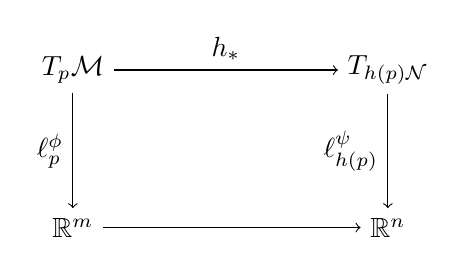
\begin{tikzpicture}
        \node (tpm) at (0, 0) {$T_p\manifold[M]$};
        \node (thpn) at (4, 0) {$T_{h(p)\manifold[N]}$};
        \node (rm) at (0, -2) {$\mathbb{R}^m$};
        \node (rn) at (4, -2) {$\mathbb{R}^n$}
            edge[<-] (rm);
        \draw[->] (tpm.east) -- (thpn.west) node[midway, above] {$h_*$};
        \draw[->] (tpm.south) -- (rm.north) node[midway, left] {$\ell_p^\phi$};
        \draw[->] (thpn.south) -- (rn.north) node[midway, left] {$\ell_{h(p)}^\psi$};
    \end{tikzpicture}
\end{document}